\documentclass[notitlepage,english]{hgbreport}

\RequirePackage[utf8]{inputenc}
\usepackage{minted}
\usepackage{subfig}
\usepackage{caption}
\graphicspath{{images/}}  
\bibliography{references}

%%%----------------------------------------------------------
\author{Hanna Wagner}
\title{Accent Classification using Machine Learning\\ 
			Project Report}
\date{\today}
%%%----------------------------------------------------------


%%%----------------------------------------------------------
\begin{document}
%%%----------------------------------------------------------

\maketitle

\begin{abstract}
\noindent
Machine Learning and Artificial Intelligence are becoming more and more popular every day. Therefore the decision was made to address this current topic by trying out different algorithms for a Text classification problem. The first part of this report deals with theoretical explanations of the different types of Machine Learning Systems, the various algorithms that can be used, the different possibilities to measure performance, general challenges in Machine Learning and the fundamental steps in Text Classification. The second part explains the four major steps, Research, Data Mining, Algorithms and Validation with the program code explained. Conclusively it will be shown which algorithms performed the best, what the overall résumé is and which challenges needed to be overcome.

\end{abstract}


%%%----------------------------------------------------------
\tableofcontents
\listoffigures
\listoftables
%%%----------------------------------------------------------

%%%----------------------------------------------------------
\chapter{Aims and Context}
%%%----------------------------------------------------------
The purpose of this semester project is to get a good basic knowledge in machine learning. Because there is no prior knowledge in this field the decision was to get familiar with Text Classification, which is one of the fundamental parts of machine learning. 
\newline \newline
Within this project the Dataset 20-Newsgroup\footnote{https://www.kaggle.com/crawford/20-newsgroups} has been chosen. The goal is to be able to assign each blog entry to the correct Newsgroup (e.g Politic, Sports) with a accuracy of at least 80\%. The Tool Scikit-Learn\footnote{http://scikit-learn.org} which supports Machine Learning with the programming language Python\footnote{https://www.python.org/} will be used within this project.
\newline \newline
The main challenges are not only to gain the necessary knowledge in the field of machine learning, but also the precise choices within the project. Therefore the preparation of the data in the best way possible (Data Mining), the choice of the right algorithms to predict where the data belongs to and to make a good Validation of the output, will be essential.

%%%----------------------------------------------------------
\chapter{Machine Learning Introduction}
\label{chap:Introduction}
%%%----------------------------------------------------------

Machine Learning is a relevant and very interesting field and with new algorithms and frameworks developed and improved, it is more relevant than ever. So this chapter gives an introduction into the field of Machine Learning. The following cite gives a good and understandable definition \cite{expertSystem}:
\begin{quote}
"Machine learning is an application of artificial intelligence (AI) that provides systems the ability to automatically learn and improve from experience without being explicitly programmed. Machine learning focuses on the development of computer programs that can access data and use it learn for themselves."
\end{quote}

\begin{figure}[ht]
	\centering
	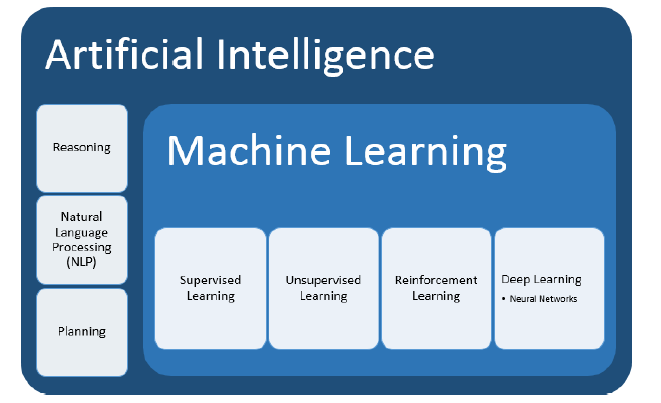
\includegraphics[width=0.7\textwidth]{images/AI_Overwiew}
	\caption{Related Fields \cite{mueller2016machine}}
\label{fig:relatedFields}
\end{figure}
\noindent Figure \ref{fig:relatedFields} shows the relation between Artificial Intelligence and Machine Learning and what other fields are dependent.

\newpage


%%%----------------------------------------------------------
\section{Types of Machine Learning Systems}
\label{sec:typesLearningSystems}
%%%----------------------------------------------------------

There are different types of Machine Learning Systems:
\begin{itemize}
\item Supervised Learning
\item Unsupervised Learning
\item Reinforcement Learning
\end{itemize}
\bigskip
Using Supervised Learning an Algorithm can be trained with an data set (input) and a solution (output). In the beginning of the training there is data with a labeled tag, which means that each dataset comes with a solution. The algorithm remembers that this dataset belongs to this special group and tries to extract some distinctive features, which should be unique for this group. The more data there is, the more features can be extracted. When there is a new dataset without a label is being put into the algorithm, it compares the unique features of the new dataset with the familiar groups that are already known. The new dataset gets the label where the highest accordance is. An exemplary task would be the classification of texts or to find out if an email is spam \cite{geron2017hands}.
\newline \newline
With the use of Unsupervised Learning Algorithms there is also a training data set (input) but does not provide a solution (output). A typical task would be to design a clustering algorithm that tries to detect e.g the groups of similar visitors on your website. Because there are no labels involved here, the program needs to find out all the characteristic and comes up with the number of groups by itself. There is also the possibility to have hierarchical clustering, which means that you can subdivide your groups into smaller ones. A possible task for these kinds of algorithms would be the anomaly detection. That means that the program could detect unusual credit card transactions\cite{geron2017hands}. 
\newline \newline
Reinforcement Learning is a little bit different compared with Supervised and Unsupervised Learning. The learning algorithm is named an agent, which discovers its environment by a trial-and-error principal. For every move the system get and reward or a penalty and it must learn by itself which the best strategy is to maximize the rewards \cite{geron2017hands}. 
\newline \newline
There are a lot of different types of Machine Learning Algorithms, which are not covered due to pettiness within this project. Nevertheless it is inevitable to understand the concept of Supervised Learning, because this will be used for the classification of texts.

%%%----------------------------------------------------------
\section{Algorithms}
\label{sec:algorithms}
%%%----------------------------------------------------------



%%%----------------------------------------------------------
\section{Measurement of Performance}
\label{sec:MeasurementofPerformance}
%%%----------------------------------------------------------


%%%----------------------------------------------------------
\section{Challenges in Machine Learning}
%%%----------------------------------------------------------

Like in every field there are some challenges one need to overcome in order to generate a good output \cite{geron2017hands}:
\begin{itemize}
\item Quantity of Training Data
\item Nonrepresentative Training Data
\item Poor-Quality Data
\item Irrelevant Features
\item Overfitting
\item Underfitting 
\end{itemize}
\bigskip
One of the hardest parts in Machine Learning to get a lot of Training Data. Unfortunately even a very simple problem would need hundreds or better thousands of examples with which the model can be trained in order to make a good prediction. For more complex programs even millions of examples would be necessary. On top of that it is also important that the input data is of high quality and represents the scenario as best as possible \cite{geron2017hands}. 
\newline \newline
The last two points are dealing with the problems of Over- and Underfitting. Overfitting or overgeneralizing in general means that your assume from one example something for a larger group. This means that the model or program only works with the test data, but not for any new data, so it is not suitable for bigger unknown data. The opposite would be underfitting. When this problem occurs your model is to elementary and hasn't extracted the features properly, so it did not learn the underlying structure of the data well enough \cite{geron2017hands}.

%%%----------------------------------------------------------
\chapter{Project Accent Classification}
\label{chap:accentClassification}
%%%----------------------------------------------------------

This chapter will describe our project steps and will show code examples of our final product. At the beginning of the project four Milestones have been identified, which will be described within the following sections. The milestones are based on the Machine Learning Cycle which is shown in Figure \ref{fig:learningCycle}.

\begin{figure}[ht]
	\centering
	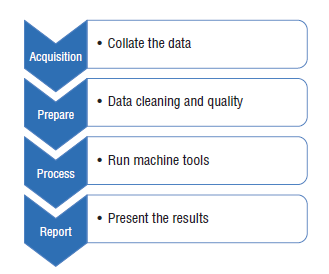
\includegraphics[width=0.65\textwidth]{images/learningCycle}
	\caption{The Machine Learning Cycle \cite{bell2014machine}}
\label{fig:learningCycle}
\end{figure}
\noindent The dataset for this project is called "20-Newsgroup"\footnote{https://www.kaggle.com/crawford/20-newsgroups} which can be downloaded from the Website Kaggle. In addition the framework Scikit-Learn\footnote{http://scikit-learn.org} which supports Machine Learning with the programming language Python\footnote{https://www.python.org/} has been used within this project.

%%%----------------------------------------------------------
\section{Research}
%%%----------------------------------------------------------

As a conclusion of our general research, which is explained in detail in \ref{chap:Introduction}, we defined our program as the following: 

\section{Data Mining}
\label{sec:DataMining}
%%%----------------------------------------------------------

%%%----------------------------------------------------------
\section{Algorithms}
\label{sec:algorithmsProject}
%%%----------------------------------------------------------

%%%----------------------------------------------------------
\section{Validation}
%%%----------------------------------------------------------

%%%----------------------------------------------------------
\chapter{Conclusion}
%%%----------------------------------------------------------

%%%----------------------------------------------------------
\section{Challenges}
%%%----------------------------------------------------------

%%%----------------------------------------------------------
\section{Lessons learned}
%%%----------------------------------------------------------

\appendix %%%-----------------------------------------------

%%%----------------------------------------------------------
\chapter{Final Code}
%%%----------------------------------------------------------

%%%----------------------------------------------------------
\MakeBibliography[nosplit]
%%%----------------------------------------------------------


\end{document}
